\section{eo\-Survive\-And\-Die$<$ EOT $>$ Class Template Reference}
\label{classeo_survive_and_die}\index{eoSurviveAndDie@{eoSurviveAndDie}}
eo\-Survive\-And\-Die A pure abstract class, to store the howmany's  


{\tt \#include $<$eo\-Survive\-And\-Die.h$>$}

Inheritance diagram for eo\-Survive\-And\-Die$<$ EOT $>$::\begin{figure}[H]
\begin{center}
\leavevmode
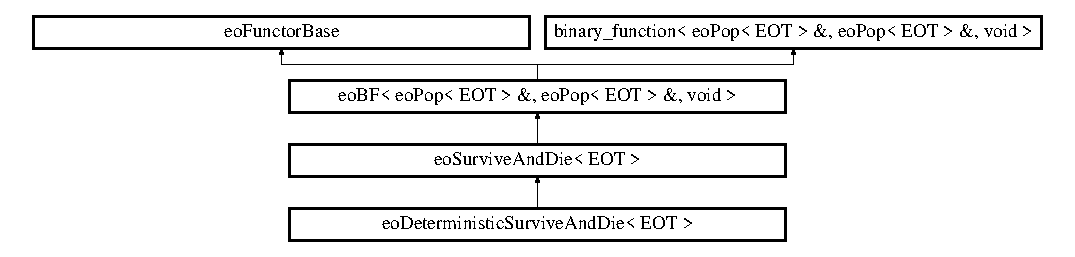
\includegraphics[height=3.01075cm]{classeo_survive_and_die}
\end{center}
\end{figure}
\subsection*{Public Member Functions}
\begin{CompactItemize}
\item 
{\bf eo\-Survive\-And\-Die} (double \_\-survive, double \_\-die, bool \_\-interpret\_\-as\_\-rate=true)\label{classeo_survive_and_die_a0}

\end{CompactItemize}
\subsection*{Protected Attributes}
\begin{CompactItemize}
\item 
{\bf eo\-How\-Many} {\bf howmany\-Survive}\label{classeo_survive_and_die_p0}

\item 
{\bf eo\-How\-Many} {\bf howmany\-Die}\label{classeo_survive_and_die_p1}

\end{CompactItemize}


\subsection{Detailed Description}
\subsubsection*{template$<$class EOT$>$ class eo\-Survive\-And\-Die$<$ EOT $>$}

eo\-Survive\-And\-Die A pure abstract class, to store the howmany's 



Definition at line 53 of file eo\-Survive\-And\-Die.h.

The documentation for this class was generated from the following file:\begin{CompactItemize}
\item 
eo\-Survive\-And\-Die.h\end{CompactItemize}
